\documentclass{report}
\usepackage[utf8]{inputenc}

% Style and margins:
\usepackage{geometry}
\geometry{
    a4paper,
    left=30mm,
    right=30mm,
    top=25mm,
    bottom=25mm,
    twoside
}
\setlength{\parskip}{3mm}
\usepackage{url}

\usepackage{titlesec}
\titleformat{\chapter}
  {\normalfont\Huge\bfseries}{\thechapter}{1em}{}

% For figures:
\usepackage{graphicx}
\usepackage{float}
\graphicspath{ {Figures/} }
\renewcommand{\figurename}{Fig.}

% For source code:
\usepackage{listings}
\usepackage{xcolor}

\lstset{
  frame=tb,
  basicstyle=\footnotesize\ttfamily,
  language=C++,
  numbers=left,
  numbersep=5pt,
  breaklines=true
}

% Math
\usepackage{amsmath}

% Data
\title{Desarrollo de aplicación 3D multiplataforma}
\author{Daniel Barca Casafont}
\date{Junio de 2017}

%%%%%%%%%%%%%%%%%%%%%%%%%%%%%%%%%%%%%%%%%%%%%%%%%
\begin{document}

\pagenumbering{roman}
\begin{titlepage}
\maketitle
\end{titlepage}

\cleardoublepage
\tableofcontents
\cleardoublepage
\pagenumbering{arabic}

\chapter{Introducción}
\section{Motivación}
Interiorvista es una empresa especializada en la generación de imágenes por computador (mucho más baratas, rápidas y de igual o mejor calidad que las que pueden obtenerse con un plató y un fotógrafo) y en el desarrollo de aplicaciones web (que requieren personal muy especializado y una gran inversión de tiempo).

Entre estas aplicaciones se encuentran los \textit{Interiorvista Planner}, un conjunto de aplicaciones que tienen el objetivo de permitir a los usuarios generar habitaciones tridimensionales y poblarlas con los productos que los clientes ofrecen en su catálogo. Esto plantea una serie de retos a varios niveles.

En su estado actual, las aplicaciones desarrolladas tienen problemas que hacen cada vez más difícil el mantenimiento y la mejora de estas. Muchas de sus características han sido desarrolladas sin llevar a cabo ningún diseño previo, o incluso sin una especificación previa de los requerimientos de la aplicación, provocando que estos surjan a lo largo del desarrollo.

\begin{figure}[H]
    \centering
    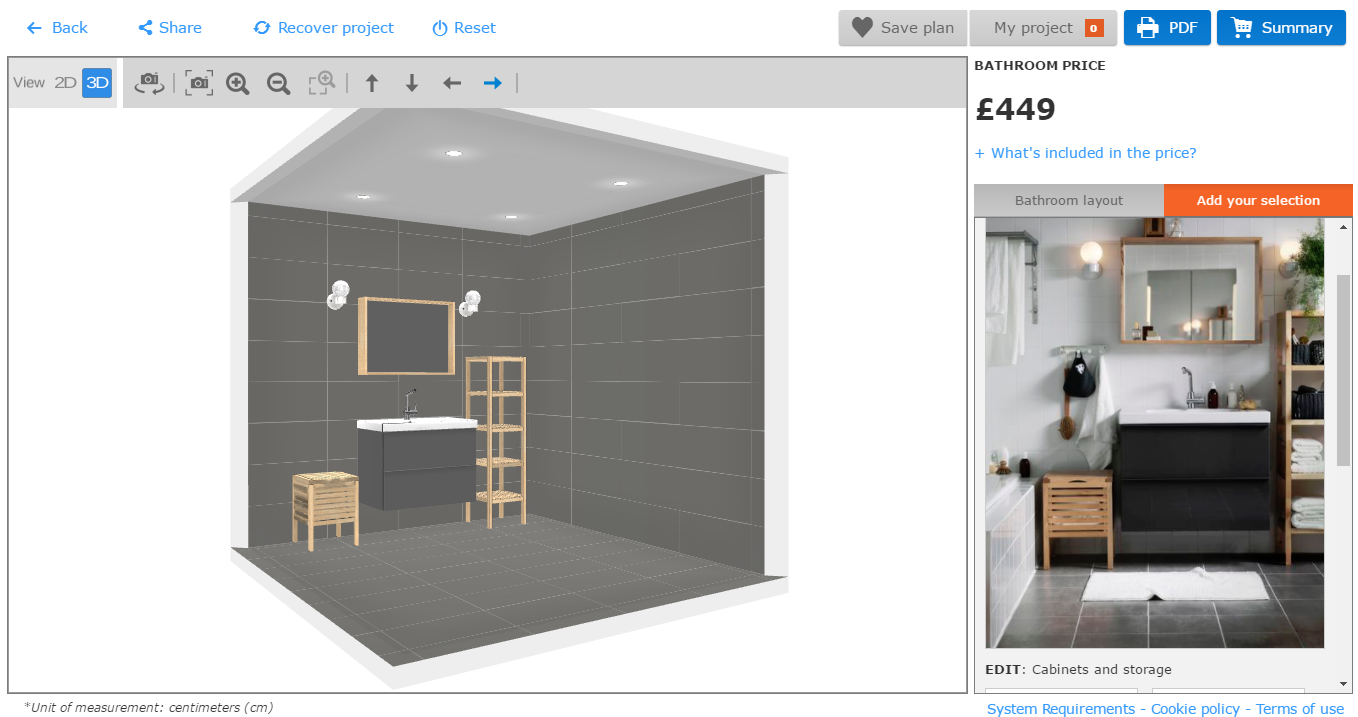
\includegraphics[width=0.8\linewidth]{bathroom_vista}
    \caption{Versión actual del planificador Bathroom Vista en vista 3D.}
    \label{fig:bathroom_vista}
\end{figure}


Las compañías de interiorismo suelen tener una serie de normas por las cuales ciertos elementos estructurales no pueden introducirse en ciertas combinaciones o en ciertas posiciones. Esto ha llevado a un código demasiado especializado en el que se introducen excepciones y condiciones arbitrarias sin mucho orden.

Se suelen requerir diversas aplicaciones muy similares para los distintos ambientes que ofrecen en su catálogo: habitaciones, comedores, baños, cocinas, etc. Aunque cada caso tiene sus particularidades, en general la mayoría de planificadores tienen suficientes características comunes como para poder tener un núcleo común, cosa que no está ocurriendo en estos momentos.

Generalmente casi siempre vamos a tener una habitación con ventanas, puertas, y una serie de elementos interiores que podemos distribuir por esta. Por ello, con un diseño efectivo debe ser posible reducir la especialización de cada una de estas aplicaciones. En el futuro, una posibilidad con la que se ha soñado en Interiorvista es la de hacer un planificador completo de una planta, con todas sus habitaciones, algo que no resultaría sencillo de conseguir con los desarrollos de que disponemos actualmente.

Entre las características comunes de los planificadores encontramos que la mayoría disponen de un modo visualización en 2 dimensiones, pensado para configurar la estructura de una habitación, y otro en 3 dimensiones, pensado para visualizar el resultado y realizar retoques sobre este. En estos momentos estos modos se han programado como dos programas distintos con una parte 2D hecha con tecnologías web, y una 3D hecha con un motor gráfico exportado a WebGL. Es una duplicidad de esfuerzos que puede evitarse utilizando una cámara ortogonal en 3D y algunas modificaciones visuales.

\begin{figure}[H]
    \centering
    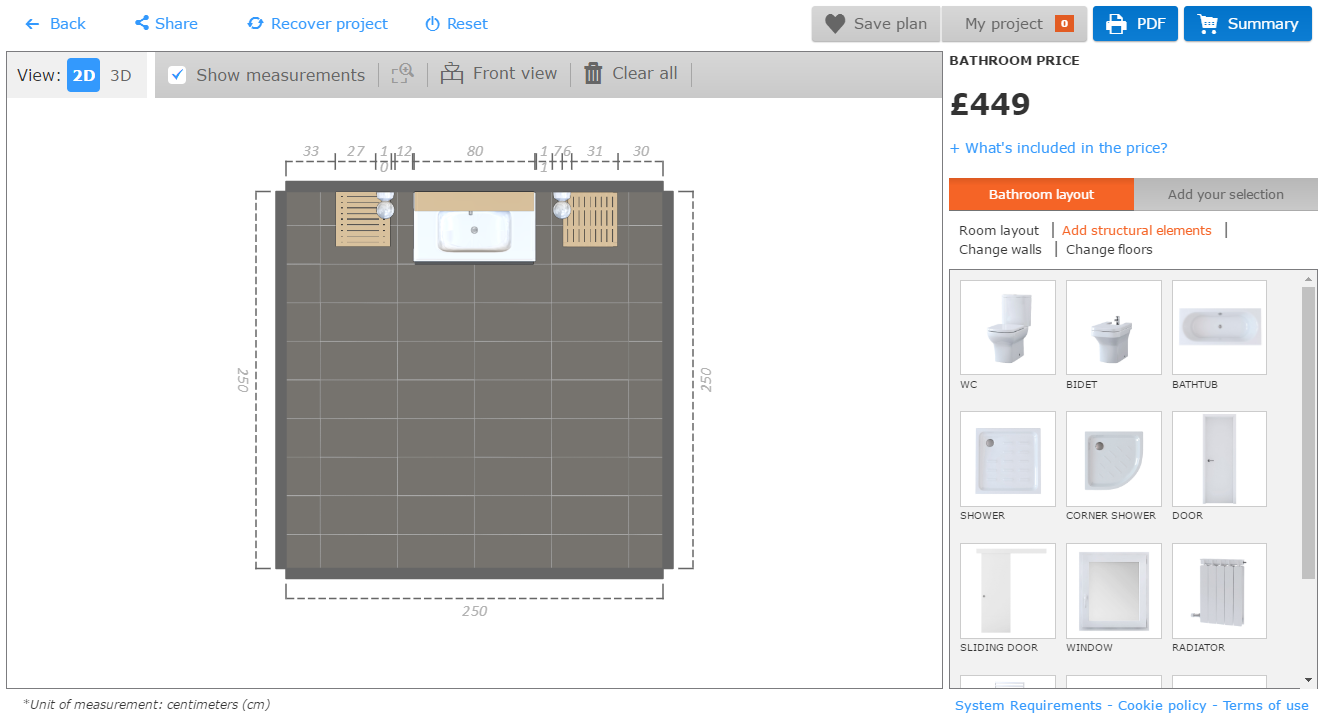
\includegraphics[width=0.8\linewidth]{bathroom_vista_2d}
    \caption{Bathroom Vista, versión en dos dimensiones del baño en la figura \ref{fig:bathroom_vista}.}
    \label{fig:bathroom_vista_2d}
\end{figure}

A pesar de las similitudes siempre hay elementos que hacen único a cada Planner: algunos baños o cocinas tienen diferentes texturas combinables para las paredes, algunas habitaciones tienen un techo inclinado o algunos productos de son altamente configurables y requieren más atención. Diferentes planificadores pueden tener un enfoque distinto: desde completas herramientas que han de poder generar y visualizar todas las configuraciones posibles de una estancia hasta aplicaciones que buscan un enfoque más emocional que atraiga a los usuarios, lo cual implica sacrificar funcionalidad en favor de la estética. Incluso pueden llegar a existir dos aplicaciones para un mismo conjunto de productos, con el objetivo de cubrir ambos puntos de vista.

El hecho de estar utilizando motores gráficos propietarios nos ha provocado problemas en el pasado. Las necesidades de la empresa son muy específicas y la imposibilidad de controlar el funcionamiento del motor ha hecho que no podamos solucionar efectivamente muchos problemas, llevándonos incluso a tener que esperar a que los desarrolladores lancen actualizaciones que arreglen nuestros problemas, o a mantener versiones abandonadas porque las versiones nuevas no son compatibles con ciertos requerimientos.

La falta de control sobre el motor gráfico también ha hecho que no pudiéramos realizar ciertas mejoras de eficiencia, visualización, o reducir el peso de la aplicación (por ejemplo, las versiones actuales incluyen toda una API de audio que no es necesaria).

\section{Objetivos}

La aplicación debe ser lo bastante genérica como para aplicarse a diferentes casos, de ahí que digamos que se trata de un conjunto de aplicaciones; y al mismo tiempo también ha de ser flexible como para dar cabida a todas estas características.

Debe contar con un visualizador en 2 y 3 dimensiones. Según el modo de visualización la interacción y las opciones son diferentes, pero el estado y la lógica de la aplicación debe mantenerse el máximo posible.

A largo plazo, la aplicación debe poder ejecutarse sobre distintas plataformas como web, escritorio, móviles o tabletas. Esto tiene muchas implicaciones a nivel de software e interacción: distintas plataformas cuentan con distintos drivers y APIs de ejecución y cada una tiene un funcionamiento y un modo de uso muy distinto. Dado que la aplicación va a estar completamente programada en C++, trasladar el código a otras plataformas (especialmente web) puede suponer un reto.

El desarrollo se realizará sobre un motor gráfico propio de la empresa, el cual está pensado para funcionar con la API gráfica Vulkan en escritorio, y debe ser adaptado para poder utilizarse con otras APIs en otras plataformas como Web o plataformas móviles. El hecho de disponer de un motor gráfico propio nos da un gran control sobre lo que ocurra dentro de este, en contraste con otras alternativas propietarias que no podemos controlar. En el pasado se han tenido muchos problemas haciendo funcionar las aplicaciones en distintas plataformas.

A nivel de diseño de software, esta es una oportunidad para repensar y reorganizar los problemas que ya conocemos. Aplicar correctamente diversas técnicas de diseño de software hará que no sólo sea más sencillo desarrollar la aplicación sino que sea más fácil de mantener y ampliar en el futuro. Algunas características son muy difíciles de implementar si no se ha seguido un cierto diseño desde el principio.

\section{Estado del arte}
Aunque existen diversos planificadores de estancias en el mercado, a día de hoy la mayoría tienen serias deficiencias y prácticamente ninguno está asociado a marcas importantes del modo en que lo está Interiorvista. Sin embargo, eso no impide que aprendamos de las alternativas existentes.

Entre los fallos más comunes se encuentran:
\begin{itemize}
    \item La necesidad de descargar aplicaciones de escritorio, o un gran número de assets que no necesariamente van a utilizarse.
    \item El uso de tecnologías obsoletas, especialmente Adobe Flash (muy popular durante la última década pero en desuso hoy en día), o motores web que requieren la instalación de plugins o extensiones.
    \item Sólo modo en 2 dimensiones o 3 dimensiones, sin la posibilidad de cambiar.
    \item Mala calidad gráfica.
    \item Interacción y/o diseño pobre.
\end{itemize}

Por supuesto, tenemos como precedente los anteriores planificadores hechos en Interiorvista, que aunque están bien situados en el mercado sufren de algunos de los fallos ya mencionados. La alternativa más sólida para lo que queremos realizar es Planner5D\footfullcite{planner5d}, que cumple buena parte de los requerimientos que queremos cumplir; sin embargo a día de hoy también tiene defectos en estabilidad e interacción, como que los elementos interiores no se adhieren a las paredes (a excepción de elementos estructurales de las paredes, como puertas y ventanas), o que en 2D pueden estropearse las paredes de forma relativamente fácil.

%Los planificadores de 2020\cite{2020} se caracterizan entre otras cosas por ofrecer imágenes estáticas de mayor calidad. El planificador espera a que el usuario deje de interactuar con la escena para generar la imagen y sobreponerla al canvas 3D. Aunque funciona, probablemente no se trata de la mejor aproximación a este problema, dado que el resultado no deja de ser un tanto pobre para la cantidad de trabajo que han realizado: generar un render 3D de buena calidad en la nube tiene un gran coste computacional (y por extensión, económico, pues los servidores gráficos son especialmente costosos), por lo que generar un render nuevo cada pocos segundos es inviable. Para solventarlo han reducido la calidad igualmente haciendo que, si bien se ve mejor que el render local, sigue dejando mucho que desear. Además, a nivel de interacción puede resultar engorroso notar el cambio de calidad constantemente.

%Generar imágenes de alta calidad en tiempo real no deja de ser una opción interesante, pero vale la pena considerar otras como mantener el renderizado local hasta que el usuario haya terminado de configurar su habitación, para finalmente generar una o varias imágenes de alta calidad.

\cleardoublepage
\chapter{Descripción del proyecto}
\textit{Interiorvista Planner} es una herramienta que permite crear de forma rápida y fácil el diseño de una sala a medida. Está pensada para ser genérica, de modo que después el proyecto se subdivide en otras aplicaciones.

La aplicación debe permitir configurar las dimensiones y forma de una sala para después introducir elementos propios de cada proyecto en esta, para finalmente obtener un listado de los productos introducidos, el precio de comprar dicha configuración, y un código que permite acceder al proyecto desde una tienda física para realizar la compra.

\section{Clientes}
IKEA\cite{ikea_history} es una archiconocida multinacional especializada en la venta de muebles de bajo coste. Se gestó en Suecia en el año 1943 como una tienda de venta de productos varios para el día a día a un precio reducido, y cuenta hoy con 314 tiendas repartidas en 38 países, siendo el icono más reconocible en el mundo de los muebles.

Una de las claves del éxito de IKEA es su famoso catálogo, donde los potenciales clientes podían ver los muebles que se ofertan y sus posibles distribuciones. Durante los años 2000 IKEA ha puesto su catálogo a disposición de los clientes también a través de Internet, y les ha ofrecido nuevas herramientas con las que poder imaginar cómo van a quedar los productos que compren en su hogar.

ROCA\cite{roca_history} es el principal proveedor de productos para baños del mundo. Se gestó en Gavá en 1917 como una compañía de radiadores, pero su relación con el agua hizo que se interesara rápidamente en la fabricación de porcelana en 1936 y grifería en 1954.

Al igual que IKEA, ROCA ha encontrado en internet nuevas formas de llegar a sus clientes, creando catálogos online y herramientas de configuración y visualización.

Aunque estos son los dos principales clientes de Interiorvista, la naturaleza genérica del planificador hace que cualquier empresa especializada en el interiorismo sea un potencial cliente.

\section{Objetivo del producto}
Los productos de interiorismo destacan por ser altamente configurables y modulares, para adaptarse a los gustos y necesidades de cada comprador. Esto hace que sea complejo crear una aplicación que tenga en cuenta todas las peculiaridades de los productos. Con los \textit{Interiorvista Planner} los compradores deben poder probar y visualizar las diferentes configuraciones de los productos y realizar la compra (a través del código) si así lo deciden.

Por lo tanto, el objetivo es conseguir que un máximo número de clientes generen un código y lo recuperen desde una tienda (signo de que han acabado comprado el producto). Cuanto más satisfactorio sea el proceso de configuración, más probable es que dichos clientes lleguen hasta el final, es por esto que la usabilidad y los tiempos de carga son clave.

Otro objetivo indirecto es hacer que la aplicación sea lo suficientemente genérica como para poder adaptarse, con poco esfuerzo, a los diferentes sub-proyectos.

\section{Usuarios}
Hay dos posibles usuarios de la aplicación: los compradores, que pueden acceder a esta a través de la página web del cliente, desde los ordenadores disponibles en las tiendas o bien desde las aplicaciones móviles; y los empleados del cliente (también conocidos como coworkers), que se encuentran en las tiendas vendiendo productos y ayudando a los clientes.

El enfoque para cada cliente es algo distinto. En el caso de los compradores se busca algo más rápido y emocional, que le lleve lo más rápido posible a la compra del producto. Sin embargo, para los trabajadores esta aplicación es una completa y precisa herramienta de trabajo, que ha de ser capaz de poder reflejar cualquier posible configuración.

A pesar de esto la aplicación será razonablemente similar en ambos casos, a excepción de algunos ``atajos" con los que los trabajadores podrán llegar más rápido a las secciones que les interesan.


\cleardoublepage
\chapter{Motor gráfico}
\section{APIs gráficas}
\label{APIS}

Según la plataforma en que se esté ejecutando la aplicación, se hará uso de una API gráfica u otra. Por defecto Manta ha sido desarrollado para funcionar en escritorio haciendo uso de Vulkan, pero esta API no está disponible en web, por lo que tendremos que utilizar OpenGL ES 2 y WebGL en este caso. Con este capítulo se pretende mostrar una vista general y con poco detalle de las APIs gráficas consideradas para hacer funcionar el motor en cada plataforma.

\subsection{Vulkan}
\label{vulkan_api}
Entre las diferentes APIs gráficas que existen, la tendencia actual es la de dar cada vez más control al desarrollador sobre lo que ocurre entre la aplicación y la gráfica, dando acceso de bajo nivel al hardware. Vulkan es la respuesta de software libre a esta tendencia, y una de las APIs que más tracción está recogiendo últimamente.

Al ofrecer control de bajo nivel, con Vulkan pueden realizarse muchas optimizaciones que en una API de alto nivel no sería posible realizar\footfullcite{vulkan_spec}. Vulkan facilita el uso de múltiples dispositivos de hardware con diversos propósitos (la GPU puede utilizarse también para realizar cálculos en paralelo, sin estar necesariamente renderizando) y el uso de multithreading.

Para ello Vulkan puede detectar y listar los dispositivos de hardware que se encuentran disponibles en la máquina, así como sus capacidades y especificaciones. Por cada dispositivo se crea una cola de comandos, que describen las acciones a realizar por el hardware.

Los comandos pueden tener distintos estados que permiten controlar el flujo de la aplicación, especialmente en aplicaciones multinúcleo. Dicho estado indica si el comando se ha ejecutado, está a la espera de ejecutarse o está disponible para ser ejecutado de nuevo. Por supuesto, la pipeline gráfica se ejecuta a través de dichos comandos.

En cuanto a la gestión de memoria, Vulkan asigna dos tipos de memoria al dispositivo: una mayor cantidad para los elementos con los que ha de trabajar constantemente, que cambiará lo mínimo posible, y que es inaccesible desde fuera del dispositivo; y otra menor conocida como ``staging" que permite hacer una copia de fragmentos de la memoria principal y modificarlos desde el exterior, para subirlos de nuevo a la principal posteriormente. Este paso se realiza porque es muy ineficiente que un dispositivo acceda a la memoria de la CPU y vice-versa, tanto la GPU como la CPU deben trabajar con su propia memoria y reducir al mínimo la transmisión de datos.

Al contrario que otras APIs, en Vulkan es posible utilizar multithreading. En caso de utilizarse, esto implica la necesidad de controlar la sincronía de cuanto ocurre en la aplicación, pero resulta una gran ventaja si se está dispuesto a realizar el esfuerzo, y supone un mucho mejor aprovechamiento de la CPU teniendo en cuenta que cada vez tienen más núcleos de procesador.

Como puede verse, en Vulkan la aplicación es responsable de la mayor parte de gestión en cuanto a qué debe hacer el dispositivo en cada momento. Es algo que contrasta, como se ha dicho, con la tendencia que ha existido hasta el momento de abstraer los elementos descritos en este apartado. 

Aunque a priori el tener más control resulta beneficioso, se debe tener especial cuidado pues la dificultad de hacer funcionar Vulkan es muy superior que con otras APIs (como OpenGL en el apartado \ref{opengl_webgl_api}), llegando al extremo en que una mala implementación en Vulkan puede dar peores resultados que su equivalente en alternativas que habrían sido mucho más simples de implementar.

\subsection{OpenGL ES 2 y WebGL}
\label{opengl_webgl_api}
En estos momentos en las tecnologías web, WebGL es la única API 3D estándar y por lo tanto que vale la pena considerar. Por eso Vulkan sólo se va a utilizar en escritorio. En el capítulo \ref{emscripten_gapi} se explicará como hacer que una aplicación programada con Vulkan pueda trabajar con WebGL al cambiar a la plataforma web.

OpenGL nació en 1992 como alternativa a las APIs gráficas propietarias del momento. La especificación y estandarización hicieron que se popularizara hasta ser la API gráfica más popular \footfullcite{opengl_hist}. OpenGL ES es una versión de OpenGL para dispositivos embebidos.

WebGL apareció de la necesidad de tener un estándar de aceleración gráfica dentro de las tecnologías web. Hasta el momento las alternativas pasaban por el uso de plugins como Adobe Flash\footfullcite{stage3D_flash}. Está basado en OpenGL ES 2 y su especificación es prácticamente idéntica, de ahí que resulte relativamente sencillo convertir llamadas a OpenGL en llamadas a WebGL.

Al contrario de lo que ocurría con Vulkan en el apartado \ref{vulkan_api}, OpenGL está pensado para proporcionar la mayor sencillez de uso posible, en detrimento del control que posee el desarrollador sobre lo que ocurre a bajo nivel. En OpenGL no es necesario especificar qué dispositivo utilizar (de hecho es prácticamente imposible escoger el dispositivo, lo cual puede ser una desventaja), gestionar la memoria, o manejar los comandos ejecutados por el dispositivo.

Aunque técnicamente es posible hacer programas con múltiples hilos de ejecución con OpenGL, hacerlo no supone ninguna mejora en términos de eficiencia y supone un esfuerzo fútil\footfullcite{opengl_multithreading}. En cualquier caso, la imposibilidad de usar hilos de ejecución en Javascript hace que no podamos aprovechar multithreading de ningún modo con WebGL (véase el apartado \ref{init_emscripten} donde se explican, entre otras cosas, algunas características de Javascript).

El resultado es una mayor rapidez de desarrollo y un código mucho más ligero y sencillo de estructurar en comparación con Vulkan, en consecuencia más fácil de mantener. A pesar de sus limitaciones, por lo general es suficiente para la mayoría de aplicaciones 3D. Para aplicaciones en las cuales el rendimiento sea crítico, sus limitaciones pueden llegar a ser un problema, o al menos una desventaja importante.

\subsection{Otras plataformas}
Aunque en este documento sólo se profundiza en el desarrollo para escritorio y web, en el futuro se espera poder exportar a otras plataformas como sistemas operativos móviles. En este área hay algunas diferencias entre los diferentes proveedores de dispositivos móviles.

A día de hoy, dispositivos con iOS de Apple son compatibles con las versiones de OpenGL ``OpenGL ES 1.1", ``OpenGL ES 2.0" y ``OpenGL ES 3.0" \footfullcite{apple_dev_opengl} mientras que en Android de Google se acepta ``OpenGL ES 1.0", ``OpenGL ES 2.0", ``OpenGL ES 3.0" y ``OpenGL ES 3.1" \footfullcite{google_dev_opengl}. Cada versión de OpenGL tiene ciertas características que mejoran a la anterior aunque hacer uso de estas suele dar problemas de incompatibilidad con las anteriores (las versiones previas de cada sistema operativo puede tener menos versiones de OpenGL compatibles).

Android dispone de una versión de Vulkan pensada especialmente para dispositivos móviles\footfullcite{android_vulkan}, por lo que la exportación de código a Android debería ser relativamente directa. iOS en cambio dispone de su propia API para gráficos de bajo nivel: Metal. Metal comparte gran parte de la filosofía de Vulkan, pero realizar la exportación podría implicar bastante más esfuerzo. No hay expectativas de que Apple incluya soporte a Vulkan dentro de iOS a corto plazo.

Microsoft también cuenta con su propia API gráfica, DirectX, aunque los dispositivos móviles con Windows representan hoy en día una parte marginal del mercado, y es poco probable que valga la pena el esfuerzo de portar el código. Al igual que Vulkan y Metal, DirectX tiene un planteamiento de bajo nivel, aunque su trayectoria es mucho más larga que los dos primeros (su primera versión data de 1995), y sus versiones anteriores no contaban con esta filosofía. DirectX tiene una mayor compatibilidad con dispositivos de escritorio que Vulkan, por lo que podría llegar a ser necesario portar el código a DirectX si en algún momento se requiere ejecutar en un dispositivo Windows que no acepte Vulkan (algunos clientes usan dispositivos muy específicos).

\section{Gestión de memoria}

\subsection{CPU}

\subsection{GPU}

\subsection{Carga de mallas dinámicas}

\section{Diseño de software}
\section{Exportación a Web}

\subsection{Sobre Emscripten}

\subsection{Aptación de la API}

\subsection{Gestión de ficheros}

\subsection{Comunicación C++/Javascript}

\section{Exportación a otras plataformas}

\subsection{Compatibilidad de APIs gráficas}

\subsection{Compilación a escritorio}

\subsection{Compilación a plataformas móviles}
\section{Shaders}

\cleardoublepage
\chapter{Diseño}
\section{Diseño de software}

\cleardoublepage
\chapter{Desarrollo}
\section{Mallas dinámicas}
\label{walls_holes}
Uno de los principales requerimientos para un planificador es la visualización de paredes y configuración de estas para adaptarlas a las medidas de una estancia. Además, deben poderse ubicar ventanas y puertas en las paredes, lo cual afecta a la geometría de la pared dado que se debe poder ver a través de estos elementos. Para ello no es factible utilizar mallas pregeneradas, se necesita generar las paredes de forma dinámica.

En este apartado se describe el proceso de desarrollo de las paredes en 2 iteraciones, una primera en la que se crea una estructura básica para las paredes, y otra en la que se tienen en cuenta las ventanas y puertas.

%%%%%%%%%%%%%%%%%%%%%%%%%%%%%%%%%%%%%%%%%%%%%%%%%%%%%%%%%%%%%%%%%%%%%%%%%%%%%
%%%%%%%%%%%%%%%%%%%%%%%%%%%%%%%%%%%%%%%%%%%%%%%%%%%%%%%%%%%%%%%%%%%%%%%%%%%%%
%%%%%%%%%%%%%%%%%%%%%%%%%%%%%%%%%%%%%%%%%%%%%%%%%%%%%%%%%%%%%%%%%%%%%%%%%%%%%
\subsection{Generación de la estructura básica de la pared}
\label{subsec:gen1}
El primer paso ha sido crear una definición de los datos que se recibirán para describir cómo ha de ser la pared. Se trata de una lista de puntos en dos dimensiones y un valor booleano que indica si esta lista debe cerrarse conectando el último punto con el primero. Esto último es importante porque, como se puede ver en la figura \ref{fig:vertical_view_walls}, la geometría de una esquina ``suelta" es diferente a la de una esquina que conecta dos paredes entre sí.

\begin{figure}[h]
    \centering
    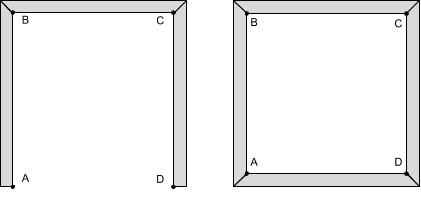
\includegraphics[width=0.65\linewidth]{Vista_Vertical_Paredes}
    \caption{Paredes en vista vertical.}
    \label{fig:vertical_view_walls}
\end{figure}

Estos datos nos permiten no sólo crear habitaciones sino también paredes únicas o incluso otros tipos de estructuras, normalmente interiores, similares a una pared. La intención es que en el futuro el programa pueda utilizarse en otras herramientas para hacer diseños más complicados como el plano de una planta completa de un edificio.

Teniendo en cuenta la estructura de una malla, explicada en el apartado \ref{mesh_light_cam}, en la figura \ref{fig:io_generatewalls} se puede ver la conversión de los datos que se espera conseguir.

\begin{figure}[H]
    \centering
    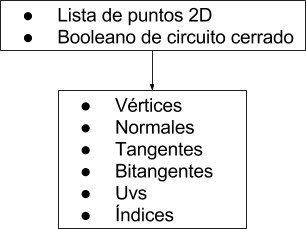
\includegraphics[width=0.5\linewidth]{IO_paredes}
    \caption{Input y output del generador de paredes.}
    \label{fig:io_generatewalls}
\end{figure}

El output está formado por listas de valores planos. Por ejemplo, la lista de vértices está formada por los valores de posición ``x,y,z" de cada uno sucesivamente.

Por cada pared hay tres primeros puntos 2D relevantes: las esquinas izquierda de las paredes anterior, actual, y siguiente. A partir de estos tres puntos puede deducirse la información de la figura \ref{fig:wall_vectors}, donde los vectores ``N1" y ``N2" son las normales de cada pared, siempre hacia el exterior de la estancia.

\begin{figure}[H]
    \centering
    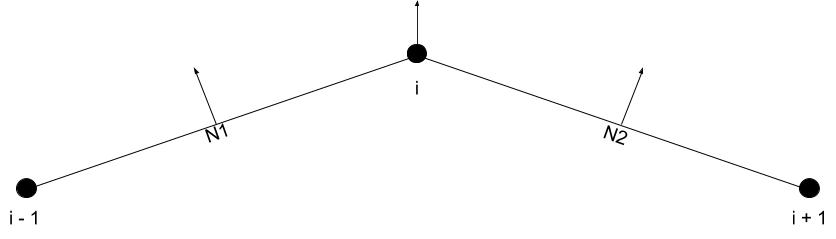
\includegraphics[width=\linewidth]{data_from_3_points}
    \caption{Vectores extraídos a partir de 3 puntos consecutivos.}
    \label{fig:wall_vectors}
\end{figure}

``N1" y ``N2" pueden obtenerse normalizando los vectores de un punto a otro, y girándolos. La dirección del vector central es la suma normalizada de estos dos o, en el caso de las paredes en los extremos cuando el circuito no está cerrado, la normal de la propia pared:

\begin{lstlisting}
VARIABLES EXTERNAS:
    puntos: lista de puntos 2D
    i: punto desde el que queremos obtener las normales de pared
    cerrado: booleano que indica si se quiere cerrar el conjunto de paredes

VARIABLE direccion TIPO VECTOR
VARIABLES v_pc, v_cn, normal_actual, normal_anterior TIPO VECTOR
VARIABLES actual, anterior, siguiente TIPO NUMERO

actual = i
anterior = i - 1

SI i EQUIVALE A tamaño(puntos) ENTONCES:
    siguiente = 0
SINO
    siguiente = i + 1
FINSI

v_pc = puntos[actual] - puntos[anterior];
v_cn = puntos[siguiente] - puntos[actual];

SI cerrado Y (actual EQUIVALE A tamaño(puntos) - 1 O actual EQUIVALE A 0) ENTONCES:
    normal_actual = GIRAR 90 GRADOS ANTI-HORARIO v_cn Y NORMALIZAR
    direccion = puntos[actual] + normal_actual
SINO
    normal_actual = GIRAR 90 GRADOS ANTI-HORARIO v_cn
    normal_anterior = GIRAR 90 GRADOS ANTI-HORARIO v_pc
    direccion = normal_actual + normal_anterior
    NORMALIZAR direccion
FINSI
\end{lstlisting}

Por último se debe tener en cuenta el grosor que se espera que tenga la pared, dado que si se avanza siempre la misma distancia en el vector director el grosor de estas dependería del ángulo que formen con sus paredes adyacentes. Esto se resuelve con trigonometría:

\begin{lstlisting}
SI cerrado ENTONCES:
    direccion = profundidad_pared / absoluto(producto_punto(normal_actual, direccion));
SINO
    direccion = profundidad_pared * normal_actual
FINSI

punto_esquina = puntos[actual] + direccion
\end{lstlisting}

El producto punto de dos vectores normales es el coseno del ángulo que forman entre sí. En este momento ``direccion" incluye la dirección y distancia entre el punto actual y el punto de la esquina exterior, permitiendo generar dicho punto a partir del actual. En el caso de que la pared que estamos generando no haga esquina con otra, simplemente se utiliza la normal de la pared actual.

Una limitación de este sistema es que los puntos deben introducirse en sentido anti-horario respecto al interior de la habitación. De lo contrario la normal de cada pared queda invertida y estas se extienden hacia el lado opuesto al que deberían, provocando algunos artefactos no deseados.

%%%%%%%%%%%%%%%%%%%%%%%%%%%%%%%%%%%%%%%%%%%%%%%%%%%%%%%%%%%%%%%%%%%%%%%%%%%%%
%%%%%%%%%%%%%%%%%%%%%%%%%%%%%%%%%%%%%%%%%%%%%%%%%%%%%%%%%%%%%%%%%%%%%%%%%%%%%
%%%%%%%%%%%%%%%%%%%%%%%%%%%%%%%%%%%%%%%%%%%%%%%%%%%%%%%%%%%%%%%%%%%%%%%%%%%%%
\subsection{Índices para la estructura básica}
Para referir a cada uno de los vértices se ha definido la nomenclatura ``A, B, A2, B2" como puede verse en la figura \ref{fig:nomenclatura_vertices}, además de los correspondientes ``AH, BH, A2H, B2H" en la parte alta de la pared. Posteriormente, los índices de la pared se extraen de los que habría normalmente en un cubo, aprovechando que sus vértices se conectan del mismo modo.

\begin{figure}[H]
    \centering
    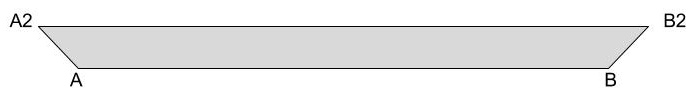
\includegraphics[width=0.75\linewidth]{Nomenclaturas_vertices}
    \caption{Nomenclatura básica de los vértices.}
    \label{fig:nomenclatura_vertices}
\end{figure}

La pared tiene 23 vértices y no 8 como cabría esperar. Esto se debe a que al renderizar, los shaders interpolan la normal de cada vértice con la de sus vecinos; si el mismo vértice se encuentra en dos caras distintas, la normal del vértice no coincide con la de la superficie en la cara que se está pintando. El resultado de esto sería que el color varía en los bordes de cada cara. Esta propiedad es muy útil para objetos que no tienen ángulos tan marcados, pero en este caso se busca que las caras sean muy marcadas y totalmente planas.

Para solucionarlo se repite cada vértice tantas veces como el número de caras en el que se encuentre, de modo que aunque todos se encuentren en la misma posición, cada cara está utilizando un vértice distinto.

\begin{figure}[H]
    \centering
    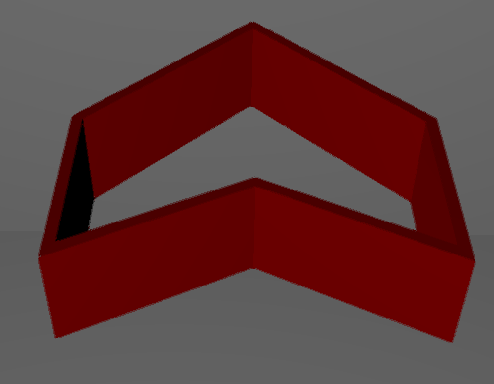
\includegraphics[width=0.75\linewidth]{paredes_first}
    \caption{Ejemplo de generación de paredes.}
    \label{fig:paredes_first}
\end{figure}

%%%%%%%%%%%%%%%%%%%%%%%%%%%%%%%%%%%%%%%%%%%%%%%%%%%%%%%%%%%%%%%%%%%%%%%%%%%%%
%%%%%%%%%%%%%%%%%%%%%%%%%%%%%%%%%%%%%%%%%%%%%%%%%%%%%%%%%%%%%%%%%%%%%%%%%%%%%
%%%%%%%%%%%%%%%%%%%%%%%%%%%%%%%%%%%%%%%%%%%%%%%%%%%%%%%%%%%%%%%%%%%%%%%%%%%%%
\subsection{Modificando la estructura para permitir la inclusión de ventanas}
\label{subsec:gen2}
El siguiente paso es implementar la posibilidad de añadir puertas y ventanas a la estancia. Insertar el modelo correspondiente en cada caso no será un problema, pero para que el efecto sea convincente es necesario poder ver a través de estos. Eso implica que se debe que modificar la geometría de las paredes para que incluya huecos donde tengan que ir dichas ventanas y puertas.

Del mismo modo que con las paredes inicialmente, se define un input: por cada hueco existe un punto 3D (que como se verá a continuación, no necesariamente debe colisionar con una pared), una altura y un ancho. El input/output del algoritmo completo para generar paredes quedaría como se puede ver en la figura \ref{fig:io_generatewindows}.

\begin{figure}[H]
    \centering
    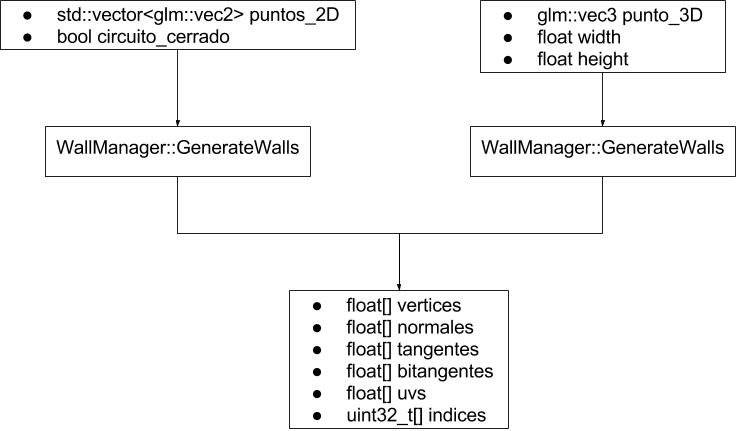
\includegraphics[width=0.75\linewidth]{I_O_ventanas}
    \caption{Nuevo input y output de GenerateWalls, incluyendo ventanas.}
    \label{fig:io_generatewindows}
\end{figure}

Para empezar se deben adaptar las paredes que ya generadas. Es conveniente que la generación de ventanas se limite a trabajar sobre un solo plano, de modo que se eliminarán los planos anterior y posterior de la pared para añadirlos después con la nueva geometría. Aunque intuitivamente pueda parecer que esto supone simplificar la geometría respecto a lo que se ha hecho hasta ahora, en realidad se complica sensiblemente. Los planos anterior y posterior de la pared van a ser siempre idénticos, pero el plano posterior es algo más alargado debido a la geometría de las esquinas que se puede apreciar en la figura \ref{fig:nomenclatura_vertices}.

\begin{figure}[H]
    \centering
    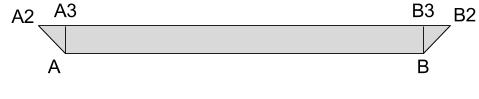
\includegraphics[width=0.75\linewidth]{Nomenclaturas_vertices_2}
    \caption{Nomenclatura final de los vértices.}
    \label{fig:nomenclatura_vertices_2}
\end{figure}

Con la nueva geometría presentada en la figura \ref{fig:nomenclatura_vertices_2} las paredes se convierten en dos prismas triangulares unidos por dos planos superior e inferior de la pared. Con esto se consigue que los planos anterior y posterior que ahora le faltan a la pared sean totalmente idénticos aunque con las normales invertidas. Esto, sin embargo, complica las conexiones entre los vértices, que se han tenido que generar manualmente. Con los nuevos vértices añadidos en total hay 35 vértices.

\begin{figure}[H]
    \centering
    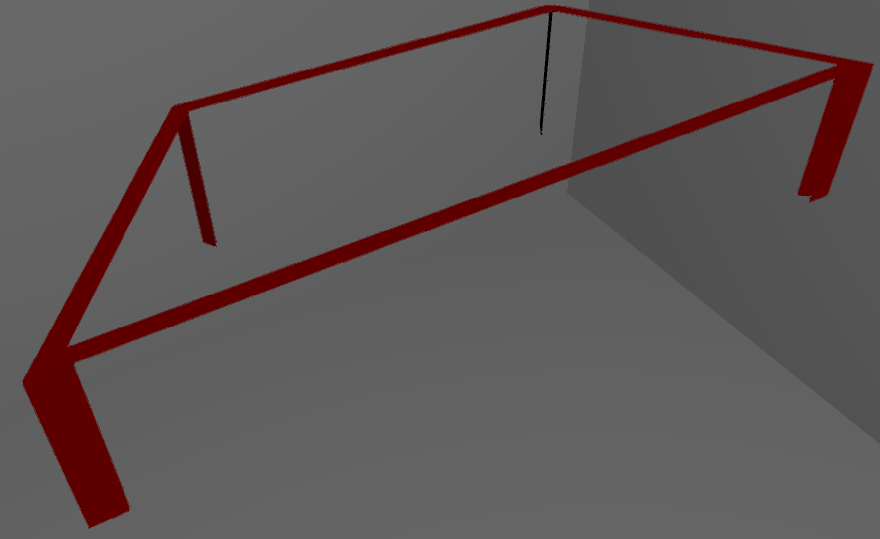
\includegraphics[width=0.75\linewidth]{paredes_frame}
    \caption{Aspecto de las paredes sin los planos anterior y posterior.}
    \label{fig:nueva_estructura}
\end{figure}

En la figura \ref{fig:nueva_estructura} puede verse el resultado. Nótese que los planos inferiores no se ven porque sus normales apuntan hacia abajo y el motor gráfico los oculta como optimización. Al crear los índices se ha tenido en cuenta el orden de estos, pues afecta al cálculo de las normales de los vértices.

%%%%%%%%%%%%%%%%%%%%%%%%%%%%%%%%%%%%%%%%%%%%%%%%%%%%%%%%%%%%%%%%%%%%%%%%%%%%%
%%%%%%%%%%%%%%%%%%%%%%%%%%%%%%%%%%%%%%%%%%%%%%%%%%%%%%%%%%%%%%%%%%%%%%%%%%%%%
%%%%%%%%%%%%%%%%%%%%%%%%%%%%%%%%%%%%%%%%%%%%%%%%%%%%%%%%%%%%%%%%%%%%%%%%%%%%%
%\clearpage
\subsection{Generación de ventanas I: proyección sobre pared}
\label{sec:wallgenwindowsi}
Como ya se ha mencionado en el apartado \ref{subsec:gen2}, las ventanas están definidas por un punto, una altura y un ancho. No se incluye ninguna información respecto a que pared es la que va a contener dicha ventana; por lo que se cogerá la pared más cercana al punto dado.

Para ello se proyecta el punto sobre la línea $AB$ de cada una de las paredes, calculando la distacia hasta cada una de las proyecciones para ver cuál es la más cercana (véase el apéndice \ref{sec:pointrayproj} sobre la proyección punto-línea):

\begin{lstlisting}
findWall(punto):
    VARIABLE pared_proxima
    VARIABLE distancia_menor
    VARIABLE distancia
    
    pared_proxima = -1
    distancia_menor = -1.0
    
    POR CADA ELEMENTO EN paredes, i:
        VARIABLE proyeccion
        proyeccion = proyeccion_punto_linea(pared[i].A1, pared[i].B1, punto)
        
        SI proyeccion encontrada ENTONCES:
            distancia = LOGITUD DE VECTOR (proyeccion - punto)
            SI distancia_menor ES MENOR QUE 0.0 O distancia < distancia_menor ENTONCES:
                distancia_menor = distancia
                pared_proxima = i
            FINSI
        FINSI
    FINPOR
    DEVOLVER pared_proxima
FIN DE FUNCION
\end{lstlisting}

Todas las ventanas o puertas han de ser necesariamente rectangulares. Esta es una precondición que se ha impuesto desde desarrollo para simplificar el cálculo de los agujeros, dado que es más sencillo incorporar geometrías más complejas incluyendo paredes falsas dentro del modelo de la ventana o puerta. Por ejemplo, si en algún momento se deseara incorporar una ventana redonda, sería más sencillo incluir 4 esquinas de pared a la ventana permitiendo que el hueco sea rectangular igualmente.

Como preparación para el próximo apartado (\ref{sec:wallgenwindowsii}) se calcula sobre la pared los 4 puntos que delimitarán la ventana. Para ello se proyecta el punto de la pared sobre el plano que forma esta, y se calcula el resto de puntos desplazándonos por dicho plano (véase el apéndice \ref{sec:pointplaneproj} sobre la proyección punto-rectángulo):

\begin{lstlisting}
projectVertices(pared, referencia a hueco):
    VARIABLE direccion_A1B1
    VARIABLE direccion_A1A1H
    VARIABLE origen
    
    direccion_A1B1 = NORMALIZAR (pared.B1 - pared.A1)
    direccion_A1A1H = NORMALIZAR (pared.A1H - pared.A1)
    
    origen = proyeccion_punto_rectangulo(pared.A1, pared.B1, pared.A1H, hueco.origen)
    
    hueco.A1 = origen
    hueco.B1 = origen + direccion_A1B1 * hueco.ancho
    hueco.A1H = origen + direccion_A1A1H * hueco.alto
    hueco.B1H = hueco.A1H + direccion_A1B1 * hueco.ancho
FIN DE FUNCION
\end{lstlisting}

%%%%%%%%%%%%%%%%%%%%%%%%%%%%%%%%%%%%%%%%%%%%%%%%%%%%%%%%%%%%%%%%%%%%%%%%%%%%%
%%%%%%%%%%%%%%%%%%%%%%%%%%%%%%%%%%%%%%%%%%%%%%%%%%%%%%%%%%%%%%%%%%%%%%%%%%%%%
%%%%%%%%%%%%%%%%%%%%%%%%%%%%%%%%%%%%%%%%%%%%%%%%%%%%%%%%%%%%%%%%%%%%%%%%%%%%%
\subsection{Generación de ventanas II: modificación de la geometría de la pared}
\label{sec:wallgenwindowsii}

Al final del apartado \ref{sec:wallgenwindowsii}, ya se conoce el punto en que están los extremos de la ventana sobre la pared. En este apartado se explica cómo dividir la pared en diferentes planos y descartar aquellos que correspondan a un agujero.

Una vez más las proyecciones cobran mucho protagonismo (véase el apéndice \ref{sec:pointrayproj} sobre la proyección punto-línea). Lo primero que se busca es dividir el plano de la pared por los vértices del hueco, obteniendo una colección de planos como se puede ver en la figura \ref{fig:wall_separacion}.

\begin{figure}[H]
    \centering
    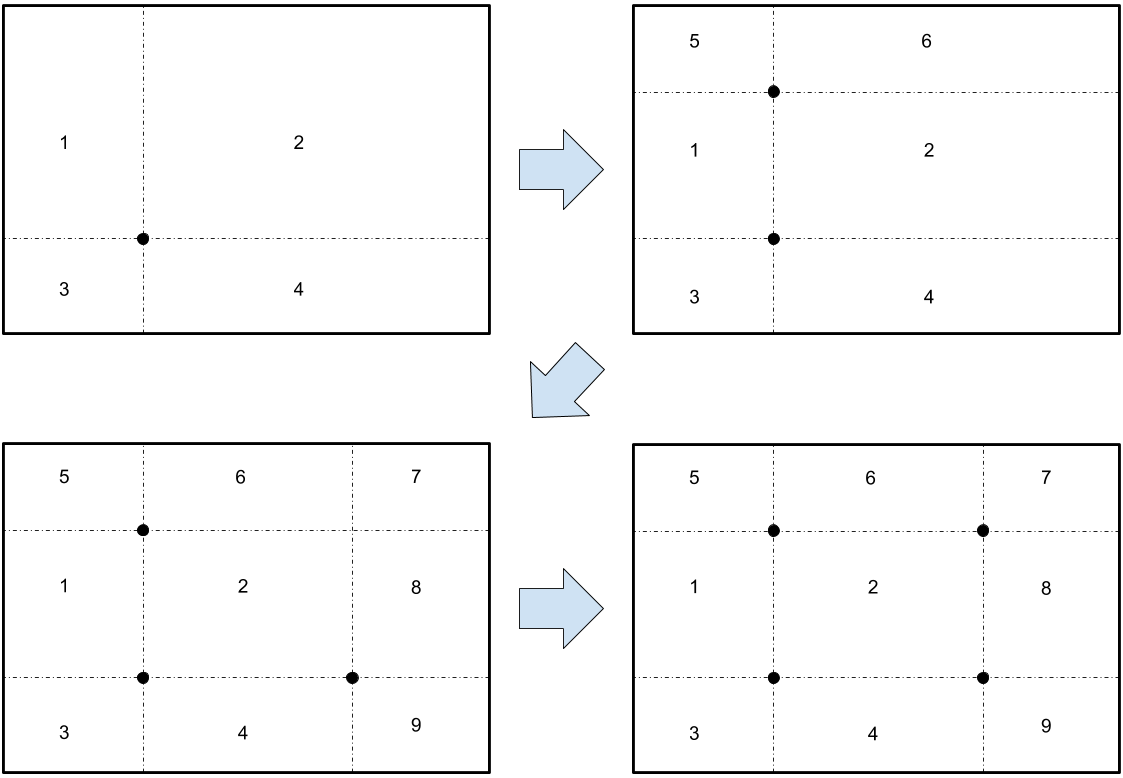
\includegraphics[width=0.85\linewidth]{Separaciones_paredes}
    \caption{Separación de la pared en planos}
    \label{fig:wall_separacion}
\end{figure}

El algoritmo para conseguir esto tiene como entrada y salida una lista de planos, que empieza siendo uno solo que cubre toda la pared. Mientras iteramos los puntos, proyectamos estos sobre cada lado para obtener los puntos por los que hay que cortar los planos, y posteriormente se añaden a la lista de planos desechando el original. En caso de que una de las proyecciones no contribuya a crear un nuevo plano (como por ejemplo, los puntos inferiores de la puerta en la figura \ref{fig:mult_and_red_windows}) la ignoramos.

Posteriormente se comprueba cuales de estos planos forman parte de una ventana y se eliminan de la lista, dejando un hueco en dicha posición. Este algoritmo permite además añadir múltiples ventanas, aumentando la posible complejidad de la pared.

Por último se reprocesan los planos generados comprobando si sus lados coinciden en alguna dirección, en cuyo caso se reúnen para reducir la complejidad. En la figura \ref{fig:mult_and_red_windows}, se puede ver un ejemplo de como se separan los planos con múltiples ventanas, y cómo se reúnen los planos adyacentes.

\begin{figure}[H]
    \centering
    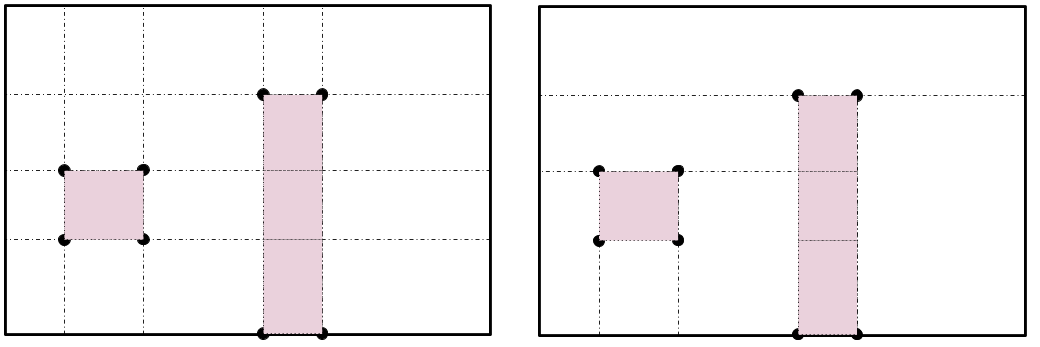
\includegraphics[width=0.85\linewidth]{mult_window_and_reduction}
    \caption{Ejemplo de pared con una ventana y una puerta, y muestra de una posible reducción de los planos.}
    \label{fig:mult_and_red_windows}
\end{figure}

\begin{figure}[H]
    \centering
    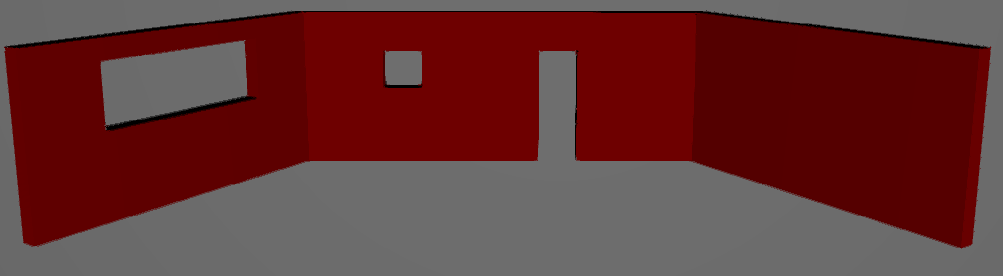
\includegraphics[width=0.85\linewidth]{Agujeros}
    \caption{Ejemplo de generación de paredes con huecos y estancia sin cerrar.}
    \label{fig:wall_with_window_example}
\end{figure}

%%%%%%%%%%%%%%%%%%%%%%%%%%%%%%%%%%%%%%%%%%%%%%%%%%%%%%%%%%%%%%%%%%%%%%%%%%%%%
%%%%%%%%%%%%%%%%%%%%%%%%%%%%%%%%%%%%%%%%%%%%%%%%%%%%%%%%%%%%%%%%%%%%%%%%%%%%%
%%%%%%%%%%%%%%%%%%%%%%%%%%%%%%%%%%%%%%%%%%%%%%%%%%%%%%%%%%%%%%%%%%%%%%%%%%%%%
\subsection{Generación de uvs}
Para que el motor aplique correctamente las texturas sobre las paredes, se requiere que las uvs estén a escala de mundo; es decir, se espera que dada una distancia entre dos vértices de la mima malla, sus uvs tengan la misma distancia. La mayor dificultad en este caso está en que los vértices se encuentran en espacio tridimensional, mientras que las uv son coordenadas bidimensionales de la textura que estamos mapeando. Por lo tanto, de algún modo hay que desconsiderar la orientación de la pared y centrarnos en sus superficies.

Como la geometría está formada por planos perfectos, la solución encontrada ha consistido en partir siempre de la esquina inferior izquierda de cada uno de ellos. Como precondición, la esquina ``A" tiene la uv (0,0).

Por lo tanto por cada plano, se ha definido la uv de la esquina inferior izquierda, y los vectores hacia los cuales ``avanzan" las componentes \texttt{x} e \texttt{y} de las uv (Fig. \ref{fig:datos_uvs}).

\begin{figure}[H]
    \centering
    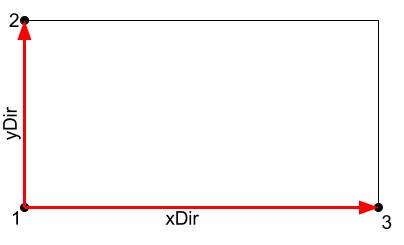
\includegraphics[scale=0.75]{Datos_uvs}
    \caption{Datos necesarios para la generación de las uv ``2" y ``3".}
    \label{fig:datos_uvs}
\end{figure}

La razón de usar proyecciones y no la magnitud de los vectores directamente, es que se desconoce en cual de las dos direcciones se encuentra el vértice que observamos al iterar. Proyectando cada punto tenemos la distancia en cada una de las dos direcciones y se la sumamos a la uv del vértice ``1":

\begin{lstlisting}
genUV(origen, xDir, yDir, punto, uv_origen, longitud_x, longitud_y):
    VARIABLE uv COMO VECTOR 2D
    uv.x = proyeccion_punto_rayo(origen, xDir, punto)
    uv.y = proyeccion_punto_rayo(origen, yDir, punto)
    
    SI longitud_x > 0.0 Y uv.x < 0.0 ENTONCES:
        uv.x = longitud_x - uv.x
    FINSI
    SI longitud_y > 0.0 Y uv.y < 0.0 ENTONCES
        uv.y = longitud_y - uv.y
    FINSI
    
    uv = uv + uv_origen
    DEVOLVER uv
FIN DE FUNCION
\end{lstlisting}

Dado que las uv no pueden ser negativas, se hace un paso en las líneas 6-11 para que, en caso de serlo, se les sume la longitud total del lado en el que se encuentran.

%%%%%%%%%%%%%%%%%%%%%%%%%%%%%%%%%%%%%%%%%%%%%%%%%%%%%%%%%%%%%%%%%%%%%%%%%%%%%
%%%%%%%%%%%%%%%%%%%%%%%%%%%%%%%%%%%%%%%%%%%%%%%%%%%%%%%%%%%%%%%%%%%%%%%%%%%%%
%%%%%%%%%%%%%%%%%%%%%%%%%%%%%%%%%%%%%%%%%%%%%%%%%%%%%%%%%%%%%%%%%%%%%%%%%%%%%
\subsection{Generación de normales, tangentes y bitangentes}
El cálculo de cada normal es el resultado de la suma de la normal de cada polígono en el que se encuentra dicho vértice, y para calcular esta se hace el producto vectorial (normalizado) de los vectores que van del primer vértice hacia el segundo y el tercero:

\begin{lstlisting}
VARIABLES EXTERNAS v1, v2, v3

normal = NORMALIZAR ( PRODUCTO CRUZADO DE (v2 - v1) Y (v3 - v1))
\end{lstlisting}

Las tangentes y bitangentes son un poco más complicadas: todo vector tiene infinitos vectores tangentes, pero en este caso no sirve cualquiera. El vector tangente a la normal tiene que estar siempre alineado con las uv.

Como se explica en el tutorial 13 de opengl-tutorial.org \footfullcite{opengltutorials}, para ello debemos resolver el siguiente sistema de ecuaciones:


\[ deltaPos1 = deltaUV1.x * T + deltaUV1.y * B \]
\[ deltaPos2 = deltaUV2.x * T + deltaUV2.y * B \]

Esto se computar como

\begin{lstlisting}
VARIABLES EXTERNAS uv1, uv2, uv3, v1, v2, v3

VARIABLES vec1, vec2
vec1 = v2 - v1
vec2 = v3 - v1

VARIABLES deltaUV1, deltaUV2 COMO VECTORES 2D
deltaUV1 = uv2 - uv1
deltaUV2 = uv3 - uv1

VARIABLE r
r = 1.0 / (deltaUV1.x * deltaUV2.y - deltaUV1.y * deltaUV2.x)

VARIABLES tangente, bitangente
tangente = (vec1 * deltaUV2 - vec2 * deltaUV1.y) * r
bitangente = (vec2 * deltaUV1.x - vec1 * deltaUV2.x) * r
\end{lstlisting}


\cleardoublepage
\chapter{Conclusiones}

\cleardoublepage
\appendix
\chapter{Utilidades matemáticas}
Normalmente un motor gráfico incluye una serie de herramientas para facilitar el desarrollo, pero debido a las carencias de nuestro motor en este aspecto, he tenido que programarlas yo mismo.

\section{Proyección punto-rayo y punto-línea}
Entendiendo un rayo como un elemento formado por un punto y una dirección y una línea como un segmento de un rayo delimitado por dos puntos, he creado las siguientes dos funciones:

\begin{lstlisting}
float point_ray_projection(glm::vec3 ray_origin, glm::vec3 ray_direction, glm::vec3 point);
bool point_line_projection(glm::vec3 line_A, glm::vec3 line_B, glm::vec3 point, glm::vec3& result);
\end{lstlisting}

Su funcionamiento es muy similar, de hecho la segunda hace uso de la primera para obtener el resultado, pero tienen dos diferencias importantes: ``point\_ray\_projection" devuelve la distancia entre el origen del rayo y la proyección de nuestro punto, en la dirección especificada, mientras que ``point\_line\_projection" devuelve un booleano que indica si la proyección está dentro de nuestra línea, y asigna a la referencia ``result" el punto exacto de la proyección.


\chapter{Patrones de diseño}
\section{Patrón componente}
\section{Patrón comando}
\section{Patrón estado}

\bibliographystyle{unsrt}
\bibliography{Bibliography}

\end{document}